\chapter{Results and Analysis}
\label{results}
In line with our objective of creating a real-time GPU ray tracer that is capable of ray tracing heterogeneous translucent materials, there are three main factors to consider when evaluating our work. The first factor is performance. In order to run at real-time frame rates, a minimum performance threshold must be met. The next factor is the size of our data set. The data must be compact enough to fit in GPU memory and still be high resolution enough such that a high quality image can be generated. Additionally, the final image quality must be considered, to determine if the renderer can correctly handle the desired visual effects, and identify any problems with our approach.

\section{Performance}
\label{sec:perf}

\begin{figure}
	\centering
	\subfloat[No effects]{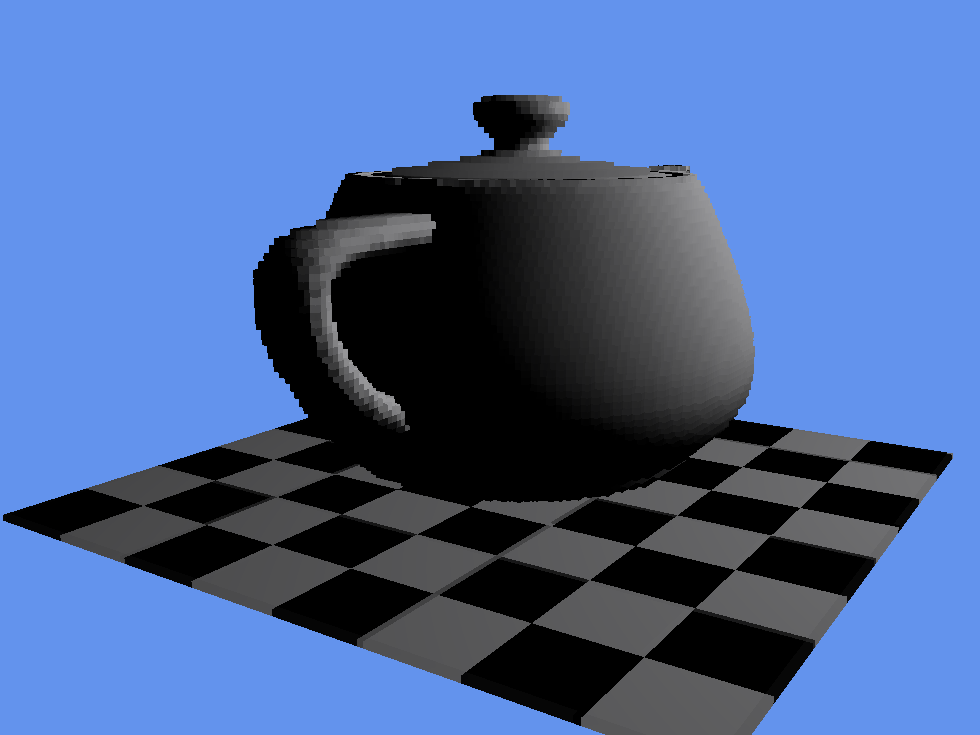
\includegraphics[width=3in]{normal_teapot.png}}
	~
	\subfloat[Shadows]{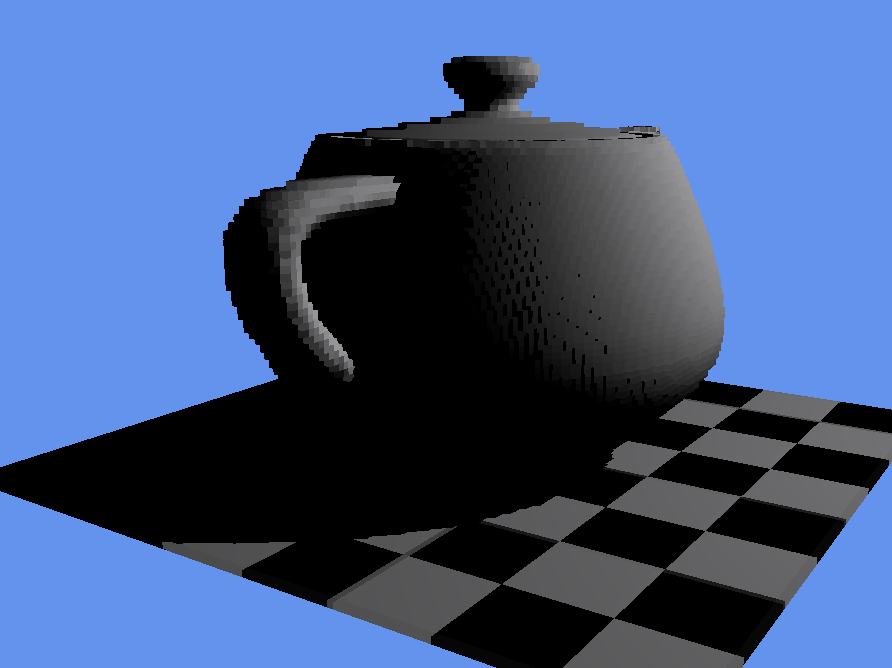
\includegraphics[width=3in]{shadow_teapot.png}}
	\\
	\subfloat[Reflection]{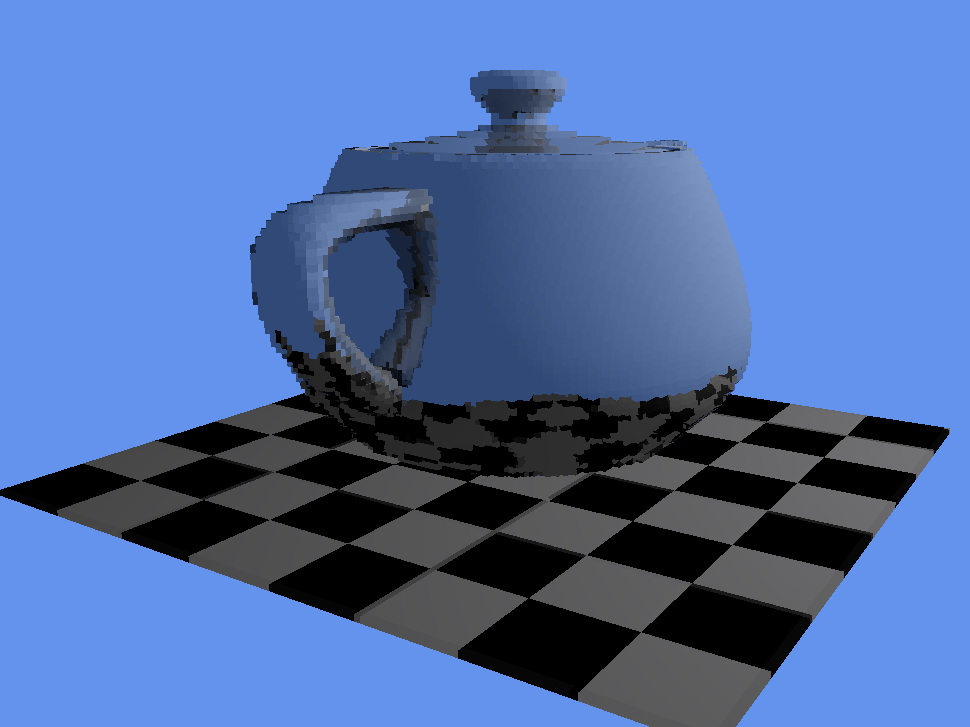
\includegraphics[width=3in]{reflective_teapot.png}}
	~
	\subfloat[Translucency]{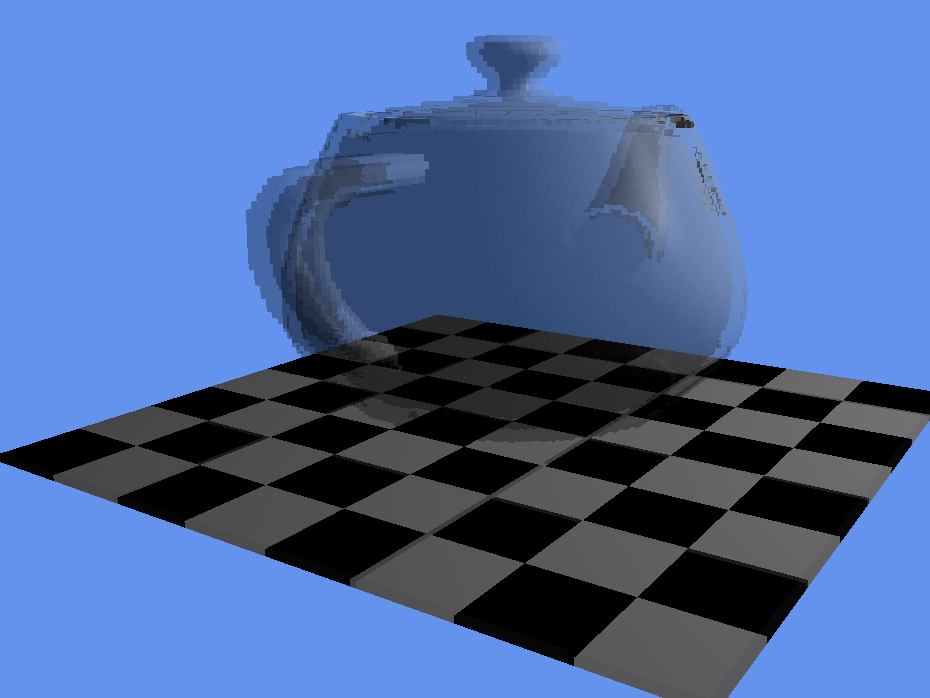
\includegraphics[width=3in]{translucent_teapot.png}}

	\caption{Our test scene at a $512^3$ resolution with various options turned on}
	\label{fig:performance-data}
\end{figure}

In evaluating the performance of our renderer there are three main criteria to consider: that it can produce reasonable quality images in real-time at high screen resolutions; that it scales well with the resolution of the data, such that the overall quality of the image produced is comparable to that of rasterisation-based renderers; and that it scales well with the resolution of the screen, such that it can be used at the higher screen resolutions desired for games.

Figure \ref{fig:performance-data} shows the resulting image from our sample scene at $512^3$ resolution with each effect enabled.

\subsection{Table of results}
\vspace{1em}

\begin{tabular}{|l|r|r|r|}
\hline

Scene \hspace{200pt} & Screen Res & Data Res & Avg FPS \\
\hline

	\quad 1 \quad		Teapot							& 768x768		& $512^2 $	&	99.34	\\
		\cline{3-4}
	\quad \quad \quad	on checker board plane			& 				& $1024^2 $	&	85.17	\\
	\cline{3-4}
														&				& $2048^2 $ &	71.55	\\
		\cline{2-4}
														& 1024x1024		& $512^2 $	&	63.05	\\
		\cline{3-4}
														& 				& $1024^2 $	&	54.45	\\
	\cline{3-4}
														&				& $2048^2 $ &	46.09	\\
		\cline{2-4}
														& 1920x1080		& $512^2 $	&	31.18	\\
		\cline{3-4}
														& 				& $1024^2 $	&	26.38	\\
	\cline{3-4}
														&				& $2048^2 $ &	22.68	\\
\hline

	\quad 2 \quad		Teapot with shadow				& 768x768		& $512^2 $	&	77.46	\\
		\cline{3-4}
	\quad \quad \quad	on checker board plane			& 				& $1024^2 $	&	65.32	\\
	\cline{3-4}
														&				& $2048^2 $ &	55.22	\\
		\cline{2-4}
														& 1024x1024		& $512^2 $	&	49.54	\\
		\cline{3-4}
														& 				& $1024^2 $	&	42.04	\\
	\cline{3-4}
														&				& $2048^2 $ &	36.10	\\
		\cline{2-4}
														& 1920x1080		& $512^2 $	&	23.24	\\
		\cline{3-4}
														& 				& $1024^2 $	&	19.40	\\
	\cline{3-4}
														&				& $2048^2 $ &	16.89	\\
\hline

	\quad 3 \quad		Reflective teapot				& 768x768		& $512^2 $	&	69.83	\\
		\cline{3-4}
	\quad \quad \quad	on checker board plane			& 				& $1024^2 $	&	58.64	\\
	\cline{3-4}
														&				& $2048^2 $ &	49.13	\\
		\cline{2-4}
														& 1024x1024		& $512^2 $	&	46.68	\\
		\cline{3-4}
														& 				& $1024^2 $	&	37.99	\\
	\cline{3-4}
														&				& $2048^2 $ &	31.93	\\
		\cline{2-4}
														& 1920x1080		& $512^2 $	&	20.44	\\
		\cline{3-4}
														& 				& $1024^2 $	&	16.88	\\
	\cline{3-4}
														&				& $2048^2 $ &	14.18	\\
\hline

	\quad 4 \quad		Translucent teapot				& 768x768		& $512^2 $	&	39.48	\\
		\cline{3-4}
	\quad \quad \quad	on checker board plane			& 				& $1024^2 $	&	32.32	\\
	\cline{3-4}
														&				& $2048^2 $ &	25.25	\\
		\cline{2-4}
														& 1024x1024		& $512^2 $	&	24.38	\\
		\cline{3-4}
														& 				& $1024^2 $	&	20.11	\\
	\cline{3-4}
														&				& $2048^2 $ &	15.96	\\
		\cline{2-4}
														& 1920x1080		& $512^2 $	&	10.07	\\
		\cline{3-4}
														& 				& $1024^2 $	&	8.30	\\
	\cline{3-4}
														&				& $2048^2 $ &	6.14	\\
\hline
\end{tabular}

\subsection{Real-time rendering}
For the purposes of our evaluation, we are defining real-time as above 30 frames per second. This is not only the minimum frame rate at which a game is expected to run, but is also above the minimum of approximately 20 required for smooth motion. Ideally, 60 frames per second is desired, as this is the refresh rate of most desktop monitors, as well as a common frame rate at which games are expected to run.

To determine if these thresholds are being met, we measure frame rate over one minute and average it.

\subsection{Scaling with screen resolution}
Our renderer is expected to perform at the high resolutions demanded by games. As our render is parallelised per pixel, in order to test how well this parallelisation functions, we have taken measurements for three screen resolutions: 768x768 (approximately 550k pixels,) 1024x1024 (approximately 1000k pixels,) and 1920x1080 (approximately 2000k pixels.) 1920x1080 was chosen as our benchmark resolution as it is at the upper bounds of standard display resolutions for video games, and as such, our renderer should be able to handle it. The lower resolutions were chosen due to an approximate doubling of pixels between each one, and as such it should allow us to determine whether our performance scales well with screen resolution.

\subsection{Scaling with data resolution}
A 3D renderer must be able to handle data of a resolution high enough to display the data smoothly. For this reason, we have chosen to measure the performance at varying data resolutions in order to determine how our methods scale with the resolution of the data.

 A $1024^3$ resolution (1024 subdivisions in each axis) was chosen as this is the resolution needed to show our data up close with similar quality to a rasterisation-based renderer. Samples were also taken at $2048^3$ and $512^3$ resolutions in order to determine how the performance is affected by varying data resolutions.

\subsubsection{Rendering with no effects (control)}
\begin{figure}[H]
\centering
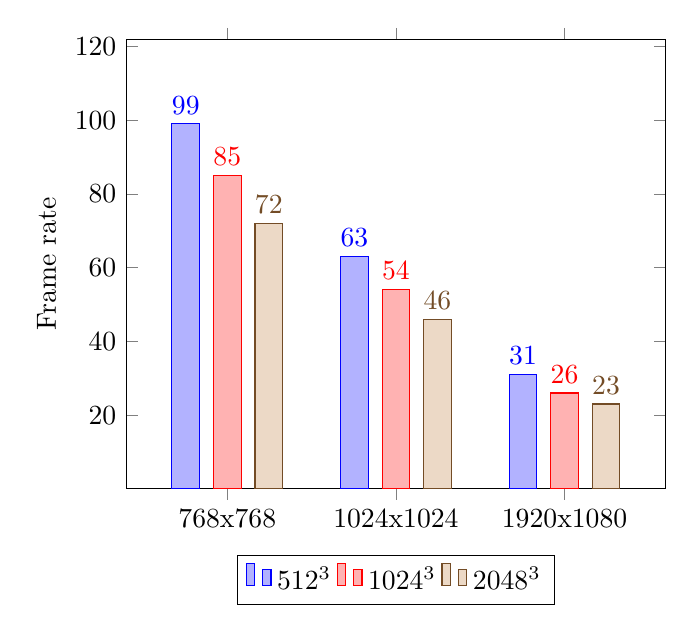
\begin{tikzpicture}
\begin{axis}[
    ybar=5pt,
    enlargelimits=0.3,
    legend style={at={(0.5,-0.15)},
      anchor=north,legend columns=-1},
    ylabel={Frame rate},
    symbolic x coords={768x768,1024x1024,1920x1080},
    xtick=data,
    nodes near coords,
    nodes near coords align={vertical},
    ]
\addplot coordinates {(768x768,99) (1024x1024,63) (1920x1080,31)}; % 512^3
\addplot coordinates {(768x768,85) (1024x1024,54) (1920x1080,26)}; % 1024^3
\addplot coordinates {(768x768,72) (1024x1024,46) (1920x1080,23)}; % 2048^3
\legend{$512^3$,$1024^3$,$2048^3$}
\end{axis}
\end{tikzpicture}

\caption{A plot of frame rate against screen resolution for our control}
\end{figure}

This data functions as our control sample, and allows us to analyse the effect on performance that different visual effects have. By examining the differences in performance with this mode of rendering, and considering the averages and ranges of these differences in performance, we can determine exactly what is affecting performance.

As shown by the graph above, our renderer exhibits a decrease in performance as the number of pixels on the screen is increased. The number of pixels increases by 78\% from 768x768 to 1024x1024, with performance decreasing by 36.0\% on average with a range of 0.94\%. For a linear decrease, one would expect the performance to increase by $100 (1 -\frac{1}{1.78}) = 44\%$, meaning that our parallelisation results in a slightly better than linear decrease in performance when the number of pixels on the screen are increased.

On the other hand, the number of pixels from 1024x1024 to 1920x1080 increases by 98\%, with performance decreasing by an average of 51.0\%, with a range of just 0.25\%. In other words, with the number of pixels on the screen doubled, the performance halves, meaning that, at high screen resolutions such as these, the performance increases linearly.

This is disappointing, and highlights a weakness in our parallelisation scheme. At higher resolutions, our renderer drops down to and below the lower end of our desired threshold for real-time rendering. With better parallelisation, one would expect a less than linear decrease in performance, with a perfectly parallelised process operating in constant time when the number of pixels is varied.

On the other hand, rendering appears to scale well with data resolution. As the resolution of the data is increased by 8 times at each step, the performance decreases by an average of 14.7\% between steps, with an average range of only 1.6\%. As such, the data structure performs very well, and should allow the rendering of a range of scenes of varying resolutions.

\subsubsection{Rendering with shadows}
\begin{figure}[H]
\centering
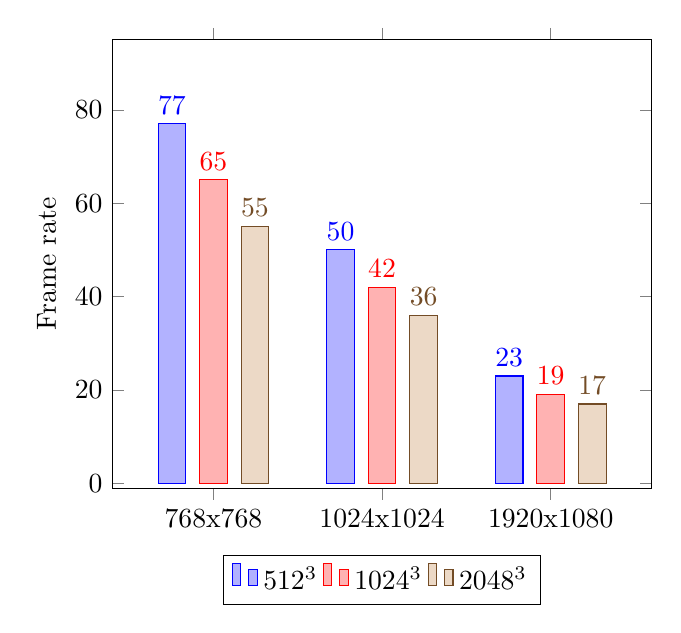
\begin{tikzpicture}
\begin{axis}[
    ybar=5pt,
    enlargelimits=0.3,
    legend style={at={(0.5,-0.15)},
      anchor=north,legend columns=-1},
    ylabel={Frame rate},
    symbolic x coords={768x768,1024x1024,1920x1080},
    xtick=data,
    nodes near coords,
    nodes near coords align={vertical},
    ]
\addplot coordinates {(768x768,77) (1024x1024,50) (1920x1080,23)}; % 512^3
\addplot coordinates {(768x768,65) (1024x1024,42) (1920x1080,19)}; % 1024^3
\addplot coordinates {(768x768,55) (1024x1024,36) (1920x1080,17)}; % 2048^3
\legend{$512^3$,$1024^3$,$2048^3$}
\end{axis}
\end{tikzpicture}

\caption{A plot of frame rate against screen resolution for rendering with shadows}
\end{figure}

As shown by the graph above, the same relationships are seen when shadows are enabled, with a minor decrease in performance. Shadow rays decrease performance by an average of 23.5\%, with a range of just 5.0\% between varying screen resolutions and data resolutions.

The range in performance decrease as screen resolution is varied ranges from 1.0\% to 1.3\%, while the same range for varying data resolutions is 3.6\% to 4.0\%, implying that data resolution is the major contributor to shadow performance. This makes sense, as the only difference between our control and shadow rendering (with reflection turned off, at least) is that a single extra ray per pixel is cast through the data. Despite this, the difference is very low, allowing the same relationships as in the control samples to show through.

Despite this decrease in performance, the performance still scales as well as the performance in our control samples, meaning that the major factors in scaling should still be the same factors as those for our control.

\subsubsection{Rendering with reflection}
\begin{figure}[H]
\centering
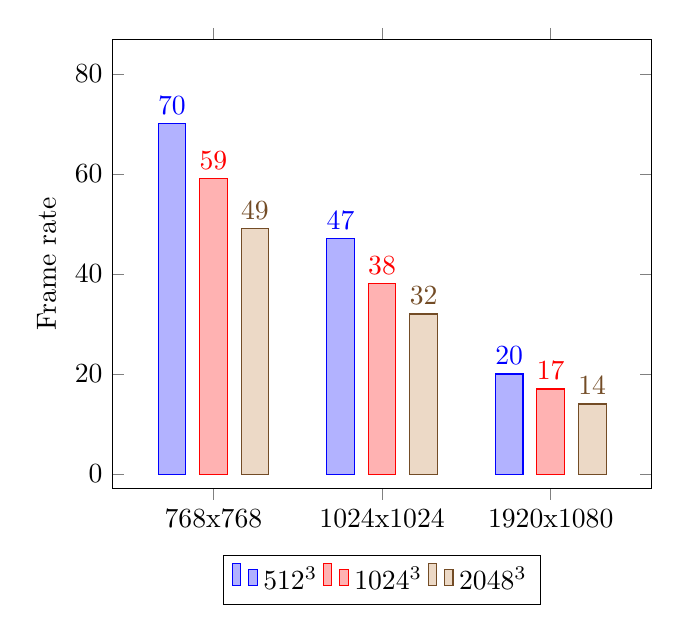
\begin{tikzpicture}
\begin{axis}[
    ybar=5pt,
    enlargelimits=0.3,
    legend style={at={(0.5,-0.15)},
      anchor=north,legend columns=-1},
    ylabel={Frame rate},
    symbolic x coords={768x768,1024x1024,1920x1080},
    xtick=data,
    nodes near coords,
    nodes near coords align={vertical},
    ]
\addplot coordinates {(768x768,70) (1024x1024,47) (1920x1080,20)}; % 512^3
\addplot coordinates {(768x768,59) (1024x1024,38) (1920x1080,17)}; % 1024^3
\addplot coordinates {(768x768,49) (1024x1024,32) (1920x1080,14)}; % 2048^3
\legend{$512^3$,$1024^3$,$2048^3$}
\end{axis}
\end{tikzpicture}

\caption{A plot of frame rate against screen resolution for rendering with reflection}
\end{figure}

Similarly to rendering with shadows, this data exhibits the same relationships as our control. This time, the average decrease in performance is 32.0\%, with a much greater overall range of 11.5\%. The performance decrease ranges from 1.6\% to 4.8\% as the screen resolution is increased, while ranging from 5.8\% to 8.5\% as data resolution is varied, indicating that, again, data resolution is the major factor affecting differences in performance of reflection.

Despite this, these ranges are still minor compared to the average difference, allowing the data to still show similar relationships to those shown by the control data.

Additionally, the performance does not seem to decrease significantly as data resolution is increased.

\subsubsection{Rendering with translucency}
\begin{figure}[H]
\centering
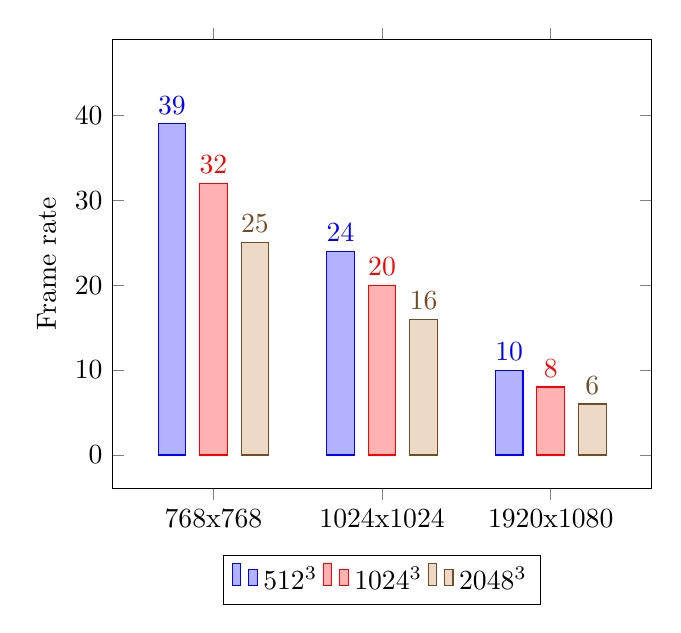
\begin{tikzpicture}
\begin{axis}[
    ybar=5pt,
    enlargelimits=0.3,
    legend style={at={(0.5,-0.15)},
      anchor=north,legend columns=-1},
    ylabel={Frame rate},
    symbolic x coords={768x768,1024x1024,1920x1080},
    xtick=data,
    nodes near coords,
    nodes near coords align={vertical},
    ]
\addplot coordinates {(768x768,39) (1024x1024,24) (1920x1080,10)}; % 512^3
\addplot coordinates {(768x768,32) (1024x1024,20) (1920x1080,8)}; % 1024^3
\addplot coordinates {(768x768,25) (1024x1024,16) (1920x1080,6)}; % 2048^3
\legend{$512^3$,$1024^3$,$2048^3$}
\end{axis}
\end{tikzpicture}

\caption{A plot of frame rate against screen resolution for rendering with translucency}
\end{figure}

This data also exhibits the same relationships as our control, but the reduction in performance is far greater when compared to shadows and reflection. The average reduction in performance for rendering our translucent object was 65.1\%, with an overall range close to that of reflection at 12.7\%. The range for varying screen resolution was 4.0\% - 5.2\%, while the range for varying data resolution was 5.5\% - 8.2\%. These are, again, not a major problem, as the data still exhibits similar relationships to the control data.

Despite this, the data for translucency shows a good relationship between performance and data resolution, with rendering scaling well as data resolution is increased. This makes sense, as our method of determining translucency is discrete, meaning it considers the volume at discrete, fixed intervals rather than the resolution of the data.

The overall decrease in performance, however, is an issue, with performance at 1920x1080 dropping into single digits. Even at lower resolutions, the performance dips below real-time frame rates.

We believe the decrease in performance comes from adding more work to the thread that renders each pixel. As more work is added to the thread, every thread must follow the most computationally expensive execution path due to the SIMD nature of the GPU. In order to address this, we believe that investigation into alternate parallelisation schemes is required.

The persistent threads technique demonstrated in \cite{aila2009hpg} seems like it could improve the parallelisation of our renderer. Firstly, the number of threads spawned on a GPU is related to achieving maximum occupancy on that GPU rather than the number of pixels on the screen, which we have shown to drop off in performance gains at higher resolutions. 

Additionally, as the processes for the initial intersection with the volume, shadows, reflection and refraction all require casting rays within the volume, we believe that it may be possible to create persistent threads that can handle any of these operations, rather than having one thread that handles all of them.

\section{Memory usage}
\label{sec:memusage}
Memory usage is an important factor to consider in real-time rendering. Ideally, all required data should be compact enough to be stored in memory. Even if this is not the case, it is desired for the memory usage to be as low as possible to reduce the amount of memory that must be considered for streaming. In order to evaluate memory usage, we have looked at the memory usage of our test scenes from section \ref{sec:perf}. Our data structure encodes volume data as well as shading data, which must be taken into account when analysing this data.

Figure \ref{fig:memory_usage} shows the memory usage of our test scene at each resolution.

\begin{figure}[H]
	\centering
	\subfloat[$512^3$ resolution, memory usage 34,354kB]{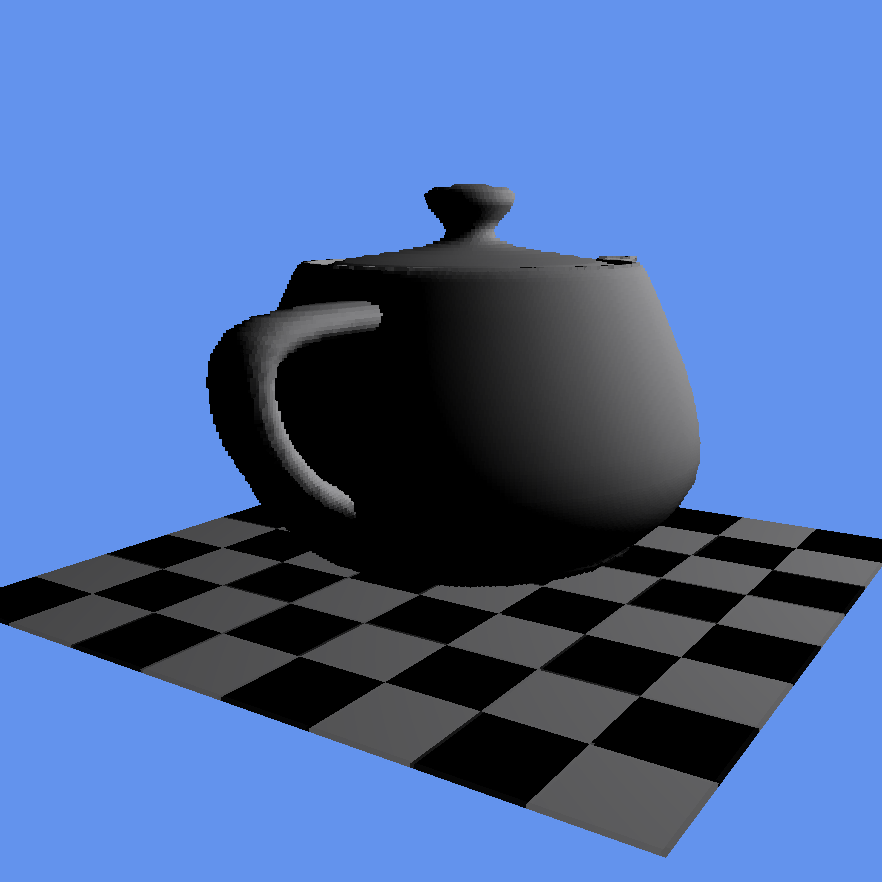
\includegraphics[width=3in]{512cubed_teapot.png}}
	~
	\subfloat[$1024^3$ resolution, memory usage 137,141kB]{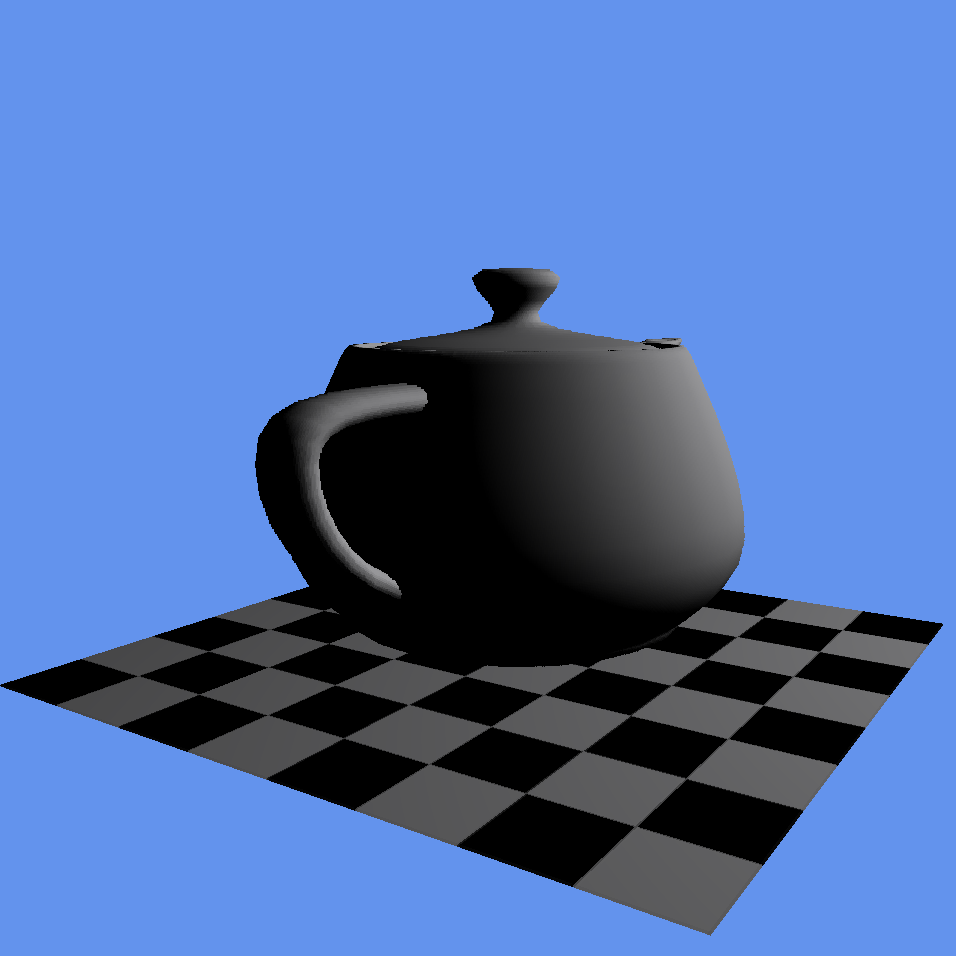
\includegraphics[width=3in]{1024cubed_teapot.png}}
	\\
	\subfloat[$2048^3$ resolution, memory usage 543,832kB]{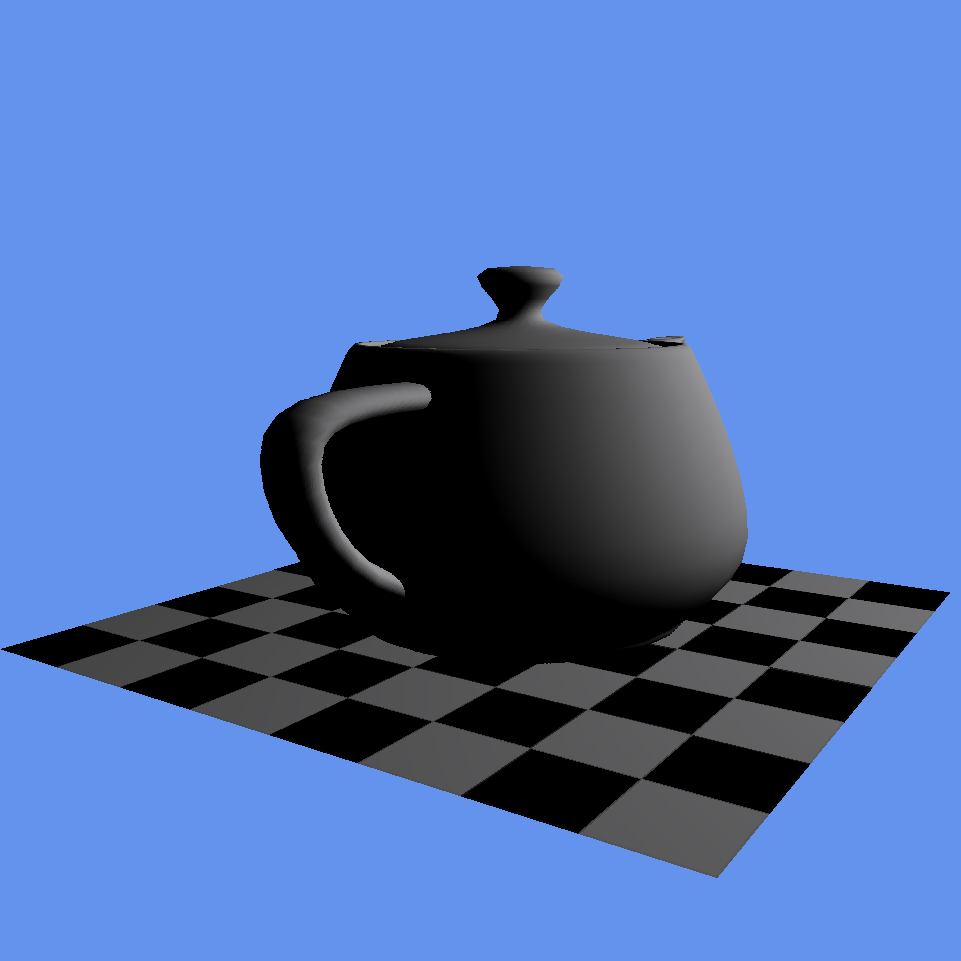
\includegraphics[width=3in]{2048cubed_teapot.png}}

	\caption{Our test scene at various resolutions and the resulting memory usage}
	\label{fig:memory_usage}
\end{figure}

As can be seen, the memory usage increases significantly for every power-of-two increase in resolution. In practice, a $1024^3$ resolution is often sufficient for smooth rendering, however up close, greater resolutions may be required. Despite the structure being compact enough to fit into GPU memory for our example scene, the memory usage is significantly greater than polygon-based meshes. Despite this structure including both volume and shading data, it still has unsatisfactorily high memory usage.

Two major approaches have been been suggested by other works to reduce the memory usage of the sparse voxel octree: contours \parencite{laine10efficientsvos}, which utilise non-cubical voxels to increase the approximation of the original data, removing the need for deeper encoding once the approximation becomes sufficient; and sparse voxel DAGs \parencite{kampe2013dags}, which allow identical regions to share pointers, and can reduce the memory usage of such structures by one to three orders of magnitude. Despite the high memory usage of our structure, these techniques should also be applicable to our work.

\section{Image quality}

\subsection{Accuracy of heterogeneous refraction}
In order to test the accuracy of our method of calculating heterogeneous refraction, we utilise two sets of data: a sphere with refractive index 1.5, with a hollow half-radius sphere embedded in it (see figure \ref{fig:half-radius-sphere}); and a sphere with refractive index 1.5, with a half-radius sphere embedded inside it of refractive index 1.0. In theory, as the refractive index of air is considered to be 1.0, the resulting images should be identical.

\begin{figure}
	\centering
	\subfloat[]{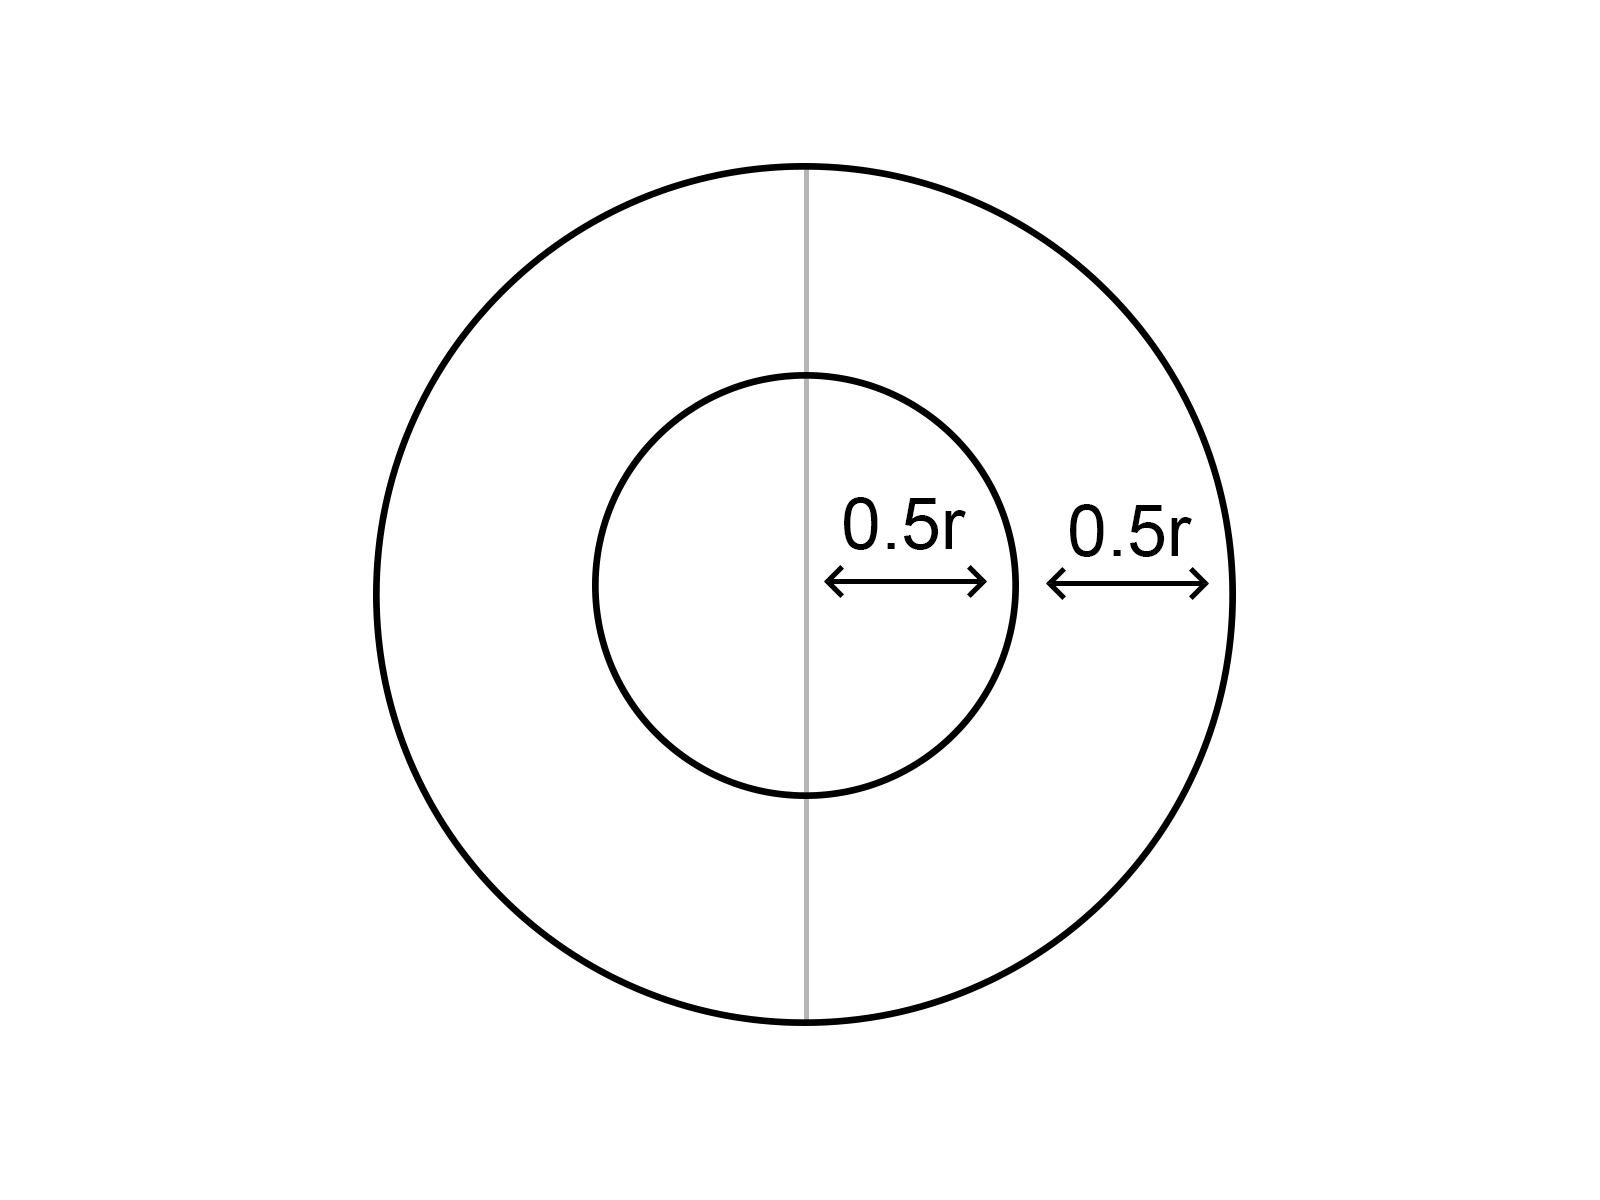
\includegraphics[width=4in]{half-radius.PNG}}

	\caption{A 2D cross section of the sphere used in this experiment. In one data set, the centre is hollow. In the other, it has a refractive index of 1.0}
	\label{fig:half-radius-sphere}
\end{figure}

\begin{figure}
	\centering
	\subfloat[Hollow centre]{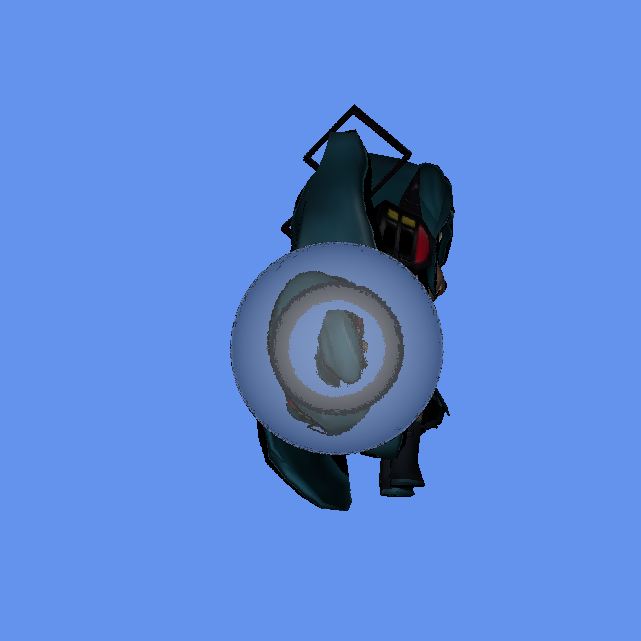
\includegraphics[width=3in]{mikuhollow.png}}
	~
	\subfloat[Refractive index 1 centre]{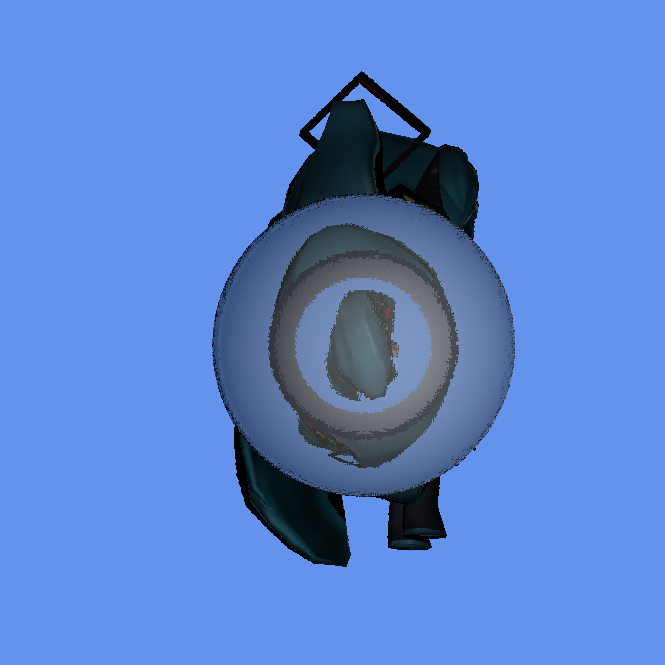
\includegraphics[width=3in]{mikunothollow.png}}

	\caption{The resulting images are identical}
	\label{fig:heterogeneous_refraction}
\end{figure}

As can be seen in figure \ref{fig:heterogeneous_refraction}, our heterogeneous refraction works as intended. It is important to note, however, that this does not prove that the result is physically accurate. Further work is required, comparing the output of our renderer to real objects that exhibit varying indices of refraction, in order to determine its physical correctness.

\subsection{Issues due to the cubical nature of voxel data}

\begin{figure}
	\centering
	\subfloat[A voxel approximation of a cube]{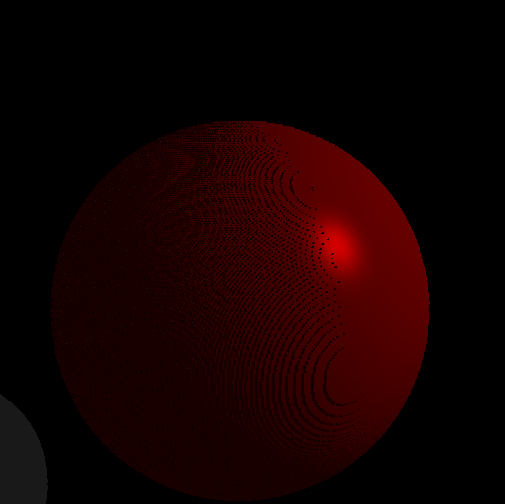
\includegraphics[width=2in]{shadowproblem.png}}
	~
	\subfloat[The phenomenon up close]{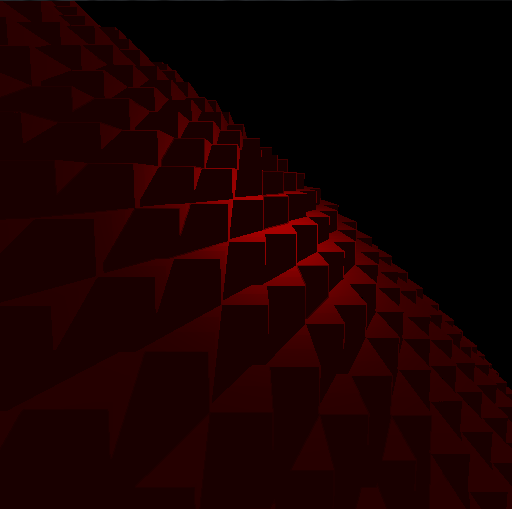
\includegraphics[width=2in]{supersmoothcube.png}}

	\caption{A voxel approximation of a cube casting shadows on itself}
	\label{fig:shadow-problem}
\end{figure}

As can be seen in figure \ref{fig:shadow-problem}, the cubical nature of voxels poses a great issue when considering secondary rays. As a sphere is a convex shape, it should, in theory, be unable to cast any shadows on its own surface. Despite this, the voxel approximation of a sphere casts shadows on itself, causing unsightly black artifacts. This problem generalises to any curved surface, as well as other types of secondary rays, such as reflection and refraction rays. Figure \ref{fig:shadow-problem-ray-path} demonstrates why this occurs, by considering the path of a shadow ray from part of the surface that is in shadow.

\begin{figure}
	\centering
	\subfloat[]{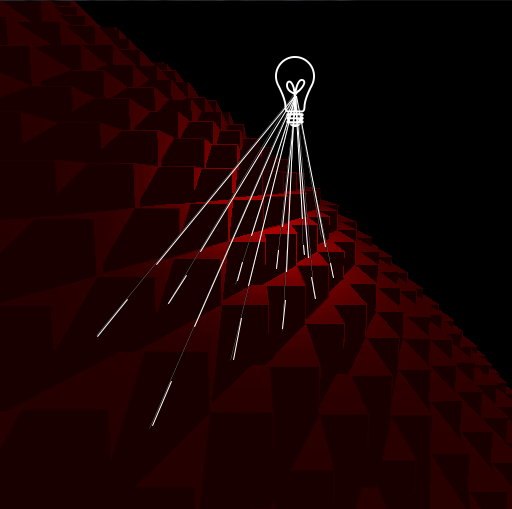
\includegraphics[width=6in]{ray_path.png}}

	\caption{The path of a shadow ray from the surface. The ray does not make it to the light, as it intersects with other voxels first}
	\label{fig:shadow-problem-ray-path}
\end{figure}

\begin{figure}
	\centering
	\subfloat[]{
\includegraphics[width=4in]{voxel_problem_reflection.PNG}}

	\caption{The problem also occurs with reflection}
	\label{fig:shadow-problem-reflection}
\end{figure}

One possible solution to this problem is to increase the data resolution. As data resolution increases, the problem lessens. The problem with this solution is that it's hard to predict, in a general way, what resolution the data will need to be stored at in order to prevent these types of artifacts in any given situation. Even lessening the effect in this way is extremely memory inefficient.

There are two main alternatives to this solution. Since the problem only occurs for surface voxels, one possible solution is to make the ray casting algorithm aware of surface normals in order to perform a sort of back-face culling. The results of this are shown in figure \ref{fig:fixed-reflection}. The major disadvantage of doing this is that it adds a number of expensive calculations to the inner loop of the ray cast, greatly reducing the overall performance of the renderer. On top of this, it would be more desirable to extend such a solution to one that does not involve considering surfaces, in order to stay in line with our volumetric rendering goals.

\begin{figure}
	\centering
	\subfloat[]{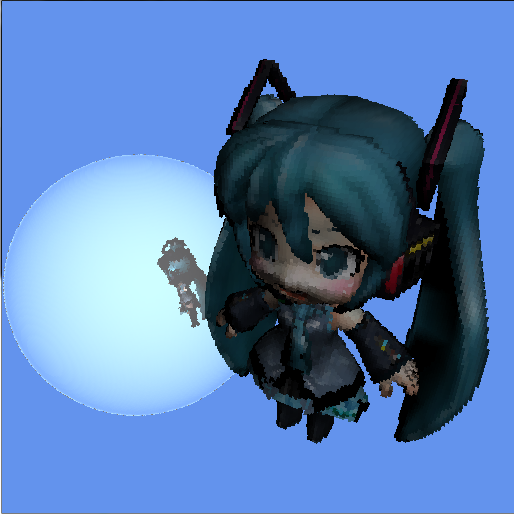
\includegraphics[width=4in]{fixed_reflection.PNG}}

	\caption{Making the ray casting algorithm aware of the normals of surfaces can solve the problem, but has disadvantages}
	\label{fig:fixed-reflection}
\end{figure}

A more generic version of this solution would use non-cubical voxels in order to improve the approximation a voxel can make of a surface. \citeauthor{laine10efficientsvos}'s contours technique, which can efficiently consider non-cubic voxels using a pair of parallel planes to bound a volume inside the voxel, does this. We believe that this technique would also solve our problems in this area, as well as greatly lessening the memory usage of our structure as discussed in section \ref{sec:memusage}.